\documentclass[../main]{subfiles}
\ifSubfilesClassLoaded{
    \dominitoc
    \tableofcontentsfile
	\pagenumbering{arabic}
    \setcounter{page}{1}
}{}
\begin{document}
\chapter{Analyse de l'auto-organisation de CxSOM}\label{chap:analyse}
\graphicspath{{06-Analyse/figures},{./figures}}
\minitoc

Cette thèse s'inscrit dans une démarche expérimentale d'analyse d'un système complexe.
Nous avons proposé un modèle de connexions de cartes auto-organisatrices au sein d'une architecture complète.
Ce modèle s'appuie sur des modèles de connexions entre cartes existant dans la littérature, utilisés notamment dans le cadre des cartes récurrentes~: la transmission de la position du BMU entre cartes.
La démarche expérimentale est constructive~: nous avons proposé un modèle d'architecture et ses règles de calcul régissant son apprentissage. Nous cherchons ensuite à identifier des comportements d'organisation en émergeant.
L'expérience présentée en exemple du chapitre représentations a permis d'identifier quelques comportements élémentaires émergeant des connexions entre cartes.

\`{A} partir des comportements que nous observerons sur plusieurs ensembles de données, nous chercherons d'abord à définir comment s'effectue l'apprentissage multimodal dans une structure de cartes.
\`{A} l'issue de ce chapitre, nous serons donc en mesure de construire des architectures de 2 et 3 cartes et d'identifier leur capacité d'apprentissage. Nous conclurons sur la scalabilité du modèle à des architectures comportant un plus grand nombre de cartes.

\section{Méthode expérimentale}

L'utilisation de modèles artificiels d'entrées nous permettent de maîtriser les dépendances entre modalités et ainsi de déterminer un lien de corrélation entre type de dépendance et organisation. Cela nous permettra également de mesurer l'apprentissage de cette dépendance connue au sein des structures de cartes.
La dépendance entre modalités est d'abord définie par la dimension choisie pour $U$. 
Une variable $U$ en une dimension paramètre des points placés sur une courbe 1D en N dimensions. $U$ en 2 dimensions paramètre un plan 2D, etc.
Ainsi, quelle que soit la dimension totale des entrées, elles sont placées sur une variété de dimension inférieure définie par $U$, apportant une dépendance entre entrées.
Les entrées considérées pour les cartes de l'architecture sont les points de dimension $N$ paramétrés par $U$. Chacune des cartes prend comme entrée un ensemble de dimensions (\emph{features}) des points.
Nous utiliserons dans les expériences suivantes des points en 2, 3, 4 et 6 dimensions. Nous étudierons les cas ou $U$ est 1D (courbes) et 2D (surfaces).

La dépendance entre entrées varie ensuite en fonction de la courbe ou surface générée, pour une même dimension de $U$.
Ensuite, pour une même dimension de $U$, la dépendance entre entrées varie.
Nous réutiliserons d'abord l'expérience présentée au chapitre représentation, sur des données disposée en cercle. L'intérêt de cette courbe est que la disposition est symétrique~: toute entrée $X^{(1)}$ correspond à deux valeurs possible pour $X^{(2)}$ et inversement.
Nous ferons varier cette propriété de dépendance en observant également le comportement de deux cartes sur des entrées identiques (cas dégénéré). Ces points sont toujours sur une courbe 1D, mais leur dépendance est bijective.
Au contraire, nous étudierons le comportement des cartes sur des entrées totalement indépendantes, prises aléatoirement dans un carré $[0,1]^n$.
Entre ces deux cas dégénérés, nous observerons le comportement d'une architecture sur des exemples implémentant des dépendances variées, par exemple si $X\m{2}$ est une fonction de $X\m{1}$.
Enfin, une carte de Kohonen classique a comme propriété d'être résistante au bruit des données. Ainsi, une carte 1D se dépliant sur un anneau fin en 2D apprendra d'abord la représentation du cercle. Nous voulons vérifier comment cette propriété se vérifie sur l'apprentissage de données par trois cartes~; nous prendrons ainsi des points sur un anneau fin.

Nous lancerons l'apprentissage de structures de deux cartes connectées réciproquement sur ces différents jeux d'entrées, comme proposé au chapitre \ref{chap:repr} et tracerons les représentations. 
Dans un premier temps, nous étudions des architectures de deux cartes 1D, ce qui nous permettra de mieux comprendre certains mécanismes d'organisation.

Nous étendons ensuite notre étude à des architectures de 3 cartes en une dimension, toutes connectées. Nous appliquerons ces architectures à une courbe ($U$ 1D) mais sur trois dimensions, chacune des cartes prenant une des dimensions d'un point comme entrée \ref{fig:cercle3}. Il s'agit ici d'un cercle en deux dimensions que nous pivotons sur la troisième dimension. De cette manière, il existe une redondance entre $X\m{1}, X\m{2}$ et $X\m{3}$ : étant donné $X\m{1}, X\m{2}$ et le modèle d'entrée, il est possible d'en déduire l'entrée manquante.
Dans ce cadre, nous réaliserons de la prédiction d'entrée par les cartes. Nous donnons en entrées $X\m{1}, X\m{2}$ à la structure et verrons si la valeur de $X\m{3}$ correspondante est correctement prédite. Une bonne prédiction témoignera de l'apprentissage du modèle d'entrées par l'architecture de cartes.

Enfin, nous étendrons notre étude à des architectures de deux et trois cartes en deux dimensions. Les entrées des cartes seront chacune en deux dimensions et situées sur une surface en dimension 4 ou 6. Nous détaillerons les équations de ces surfaces dans la section correspondante.

\begin{figure}
	\begin{minipage}{\textwidth}
		\begin{minipage}{0.33\textwidth}
			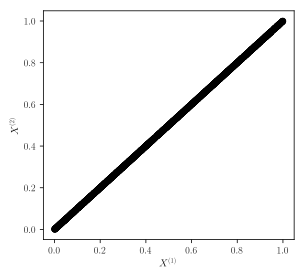
\includegraphics[width=\textwidth]{2som_id_in.pdf}
			\caption{Cas dégénéré d'entrées en deux dimensions~: $X\m{1}$ = $X\m{2}$ \label{fig:id}}
		\end{minipage}
		\begin{minipage}{0.33\textwidth}
			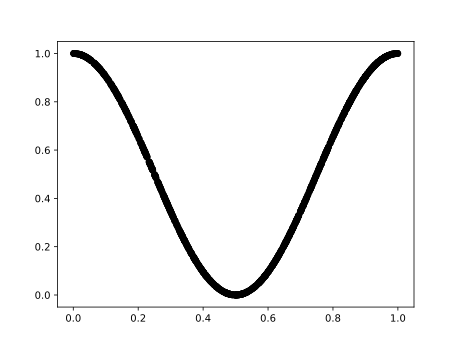
\includegraphics[width=\textwidth]{2som_courbe000_inputs.pdf}
			\caption{Cas d'entrées en deux dimensions~: $X\m{2}$ = $cos(X\m{1})$ \label{fig:cos}}
		\end{minipage}
		\begin{minipage}{0.33\textwidth}
			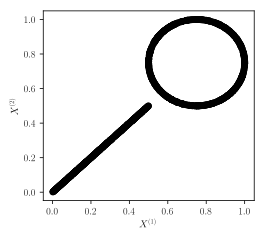
\includegraphics[width=\textwidth]{2som_mix_in.pdf}
			\caption{Exemple de dépendance en deux dimensions  \label{fig:mix}}
		\end{minipage}
	\end{minipage}
	\begin{minipage}{\textwidth}
		\begin{minipage}{0.33\textwidth}
			\includegraphics[width=\textwidth]{2som_inp_noU.pdf}
		\end{minipage}
		\begin{minipage}{0.33\textwidth}
			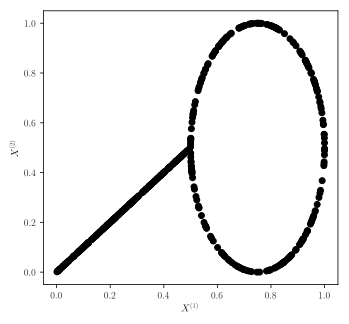
\includegraphics[width=\textwidth]{2som_mix001_in.pdf}
		\end{minipage}
		\begin{minipage}{0.33\textwidth}
			\includegraphics[width=\textwidth]{2som_square_in.pdf}
		\end{minipage}
	\end{minipage}
	
\end{figure}

\section{Quels comportements caractérisent l'apprentissage ?}

Le premier but de cette étude est d'identifier des comportements \emph{systémiques} émergeant d'une architecture simple à deux et trois cartes, sur des entrées en deux et trois dimensions.
Nous avons identifié certains comportements au chapitre précédent, que nous évaluerons sur d'autres données entrées. Nous rappelons d'abord les comportements qu'on peut attendre d'une architecture de cartes.

\subsection{Quantification vectorielle sur les entrées externes}

Une carte de Kohonen classique permet l'apprentissage de représentation sur ses entrées par quantification vectorielle. Elle extrait les structures sous-jacentes à la géométrie et topologie des points d'entrées sur un ensemble de vecteurs ordonnés.
La qualité de la quantification sur chaque carte est une première condition à vérifier pour évaluer l'organisation d'une architecture.
L'erreur de reconstruction d'une entrée par le poids de son BMU est d'abord un bon indicateur de la qualité de quantification vectorielle d'une carte~: toutes les entrées sont associées à un poids $\w\ext(\bmu)$ qui leur est proche.
Nous attendons ainsi de chaque carte de l'architecture qu'elle ait une erreur de quantification faible sur l'entrée qu'elle a appris.

\subsection{Différenciation de $U$ selon les BMUs: indicateur d'une mémoire associative}

Nous appliquons une architecture de cartes à des tâches de mémoire associative sur des entrées multimodales.
Le but de la mémoire associative est d'apprendre des données de plusieurs modalités et d'apprendre leurs associations. L'apprentissage des données indépendantes est donc un comportement nécessaire à cette mémoire associative. 
Le but de la mémoire associative est d'apprendre des relations entre les entrées. Comme une carte cherche à extraire une structure dans les données de son espace d'entrée, observe t-on l'apprentissage d'une structure dans les relations entre entrées dans l'architecture de cartes ?
Les expériences menées sur le cercle en 2D nous ont montré que les cartes s'auto-organisent de façon à ce que $U$ soit une fonction du BMU $\bmu$ dans chaque carte. Nous vérifierons cette propriété sur les nouveaux jeux d'entrées.

\subsection{Découpage d'une carte en zones grâce aux poids contextuels}

Enfin, nous remarquerons que cet apprentissage de relations passe par la disposition en zones auto-organisées au sein d'une carte. Ces zones, nous l'avons vu, déterminent la BMU de chaque carte en fonction de l'ensemble des entrées et non seulement de l'entrée de la carte en question. Ces zones ne marquent pas l'apprentissage d'une relation: dans les cas ou les entrées sont indépendantes, la carte se divise quand même en zones distinctes. La présence de zones est spécifique au comportement de l'architecture CxSOM.

\section{Architectures de 2 cartes 1D}

Analysons d'abord la forme des poids contextuels de $M\m{1}$, que nous avions tracés en figure~\ref{fig:weights} sans les commenter. Les poids externes, en orange, présentent une disposition similaire à ceux observés dans la carte classique (b). Les poids contextuels, en bleu, présentent une forme de vagues, avec 7 valeurs de maximum allant de 0.5 à 1, et 6 minimum allant de 0.5 à 0.1. Ces maximum et minimum sont répartis en zones de taille équivalente sur la carte. 

Lorsqu'on s'intéresse aux tracés des échantillons, on remarque d'abord que les positions dans la carte $M\m{1}$ se répartissent en zones étant BMUs et zones mortes, dans lesquelles aucune entrée n'a gagné. C'est une première différence avec la carte indépendante, pour laquelle toutes les positions gagneront pour des entrées. Les zones dans lesquelles il y a des BMUs correspondent aux extremum des poids contextuels et leurs alentours. C'est un phénomène inhabituel pour une carte de Kohonen. Les entrées $\inpx\m{1}$, dans la carte classique (b), correspondent à la courbe de poids externe: la valeur du poids du gagnant est toujours très proche de la valeur de l'entrée. Dans la carte $M\m{1}$, les entrées externes $\inpx\m{1}$ orange sont proches de la courbe de poids externes, mais avec plus d'erreur de quantification.
Les deux points rouge et bleu ayant la même valeur de $x$ ont un BMU différent dans la carte $M\m{1}$, alors que ces deux échantillons ont le même BMU dans la carte apprenant indépendamment sur les valeurs de $x$. Ainsi, la carte connectée au sein de CxSOM différencie les échantillons en fonction de non seulement leur entrée externe, mais aussi de l'entrée de l'autre carte de l'architecture. La plage de valeurs des $\inpx\m{1}$ gagnant dans un des zones recoupe les plages de valeurs gagnant dans les zones situées à gauche et à droite. Par exemple, la zone dans laquelle l'échantillon rouge gagne, autour de $\bmu\m{1} = 0.25$. La partie des entrées située en dessous de la courbe de poids externe recoupe les valeurs d'entrées gagnant dans la zone précédente; la partie située au dessous de la courbe de poids externe recoupe des valeurs gagnant dans la partie suivante. Pour une entrée externe, le choix de la zone de BMU dans laquelle elle gagnera dépend alors de l'entrée contextuelle. 


Dans la carte $M\m{1}$, une unité se spécialise donc par rapport aux deux entrées et non pas une seule comme dans la carte indépendante: les entrées externes et l'entrée contextuelles. C'est bien ce à quoi on s'attendait en ayant deux couches de poids. Ce qui est intéressant est que cette différenciation est réalisée par la répartition des unités en un nombre fini de zones distinctes. Dans chaque zone, les unités sont BMUs pour un segment de valeurs d'entrée externe et contextuelles. Au sein d'une zone, la répartition des entrées externe selon le BMUs est ordonnée, comme ce serait le cas dans une carte auto-organisatrice classique. Le comportement de la carte au sein d'une zone reste donc similaire à celui d'une carte classique.

Deux zones adjacentes correspondent par ailleurs à des segments de valeur d'entrée en partie superposés, et des segments de valeurs d'entrées contextuelles différentes. Il s'agit d'une deuxième échelle d'organisation, qui garde également l'aspect ordonné d'une carte classique. Ces zones sont créées par auto-organisation~; aucun paramètre de la carte n'a été modifié pendant l'apprentissage pour former ces zones, et le nombre d'unités allouées par auto-organisation dans chaque zone est à peu près égal. La carte agit un peu comme une base de données structurée avec des indices primaires et des indices secondaires pour chaque neurone, l'indice primaire étant la zone de la carte, et l'indice secondaire la position dans cette zone.

\begin{figure}
	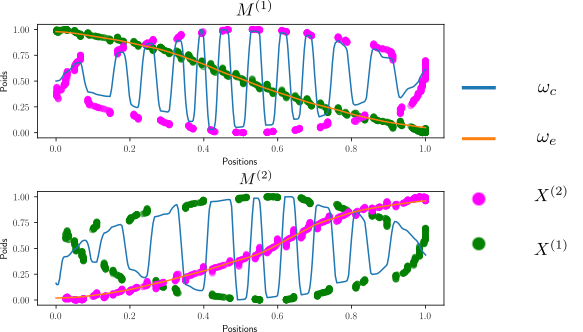
\includegraphics[width=0.7\textwidth]{2som_cercle_w.pdf}
\end{figure}

\begin{figure}
	\includegraphics[width=0.7\textwidth]{3som_cercle_w.pdf}
\end{figure}

\begin{figure}
\begin{minipage}{0.66\textwidth}
	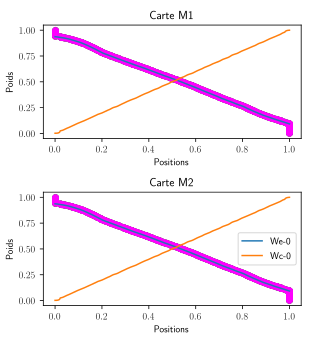
\includegraphics[width=\textwidth]{2som_id_w.pdf}
	\caption{Représentation cartographique des poids et entrées pour la disposition identité}
\end{minipage}
\begin{minipage}{0.33\textwidth}
	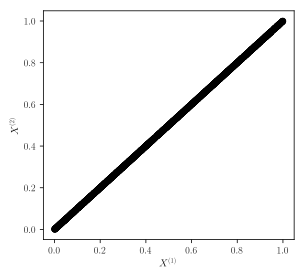
\includegraphics[width=\textwidth]{2som_id_in}
\end{minipage}
\end{figure}

\begin{figure}
	\begin{minipage}{0.66\textwidth}
	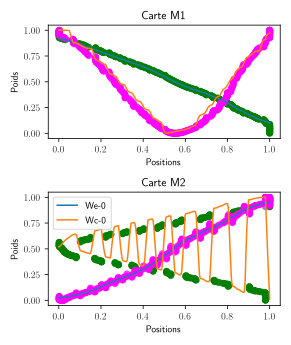
\includegraphics[width=\textwidth]{2som_cos_w.pdf}
	\caption{Représentation cartographique des poids et entrées pour la disposition cos}
	\end{minipage}
	\begin{minipage}{0.33\textwidth}
		\includegraphics[width=\textwidth]{2som_cos_in.png}
	\end{minipage}
\end{figure}

\begin{figure}
	\begin{minipage}{0.66\textwidth}
		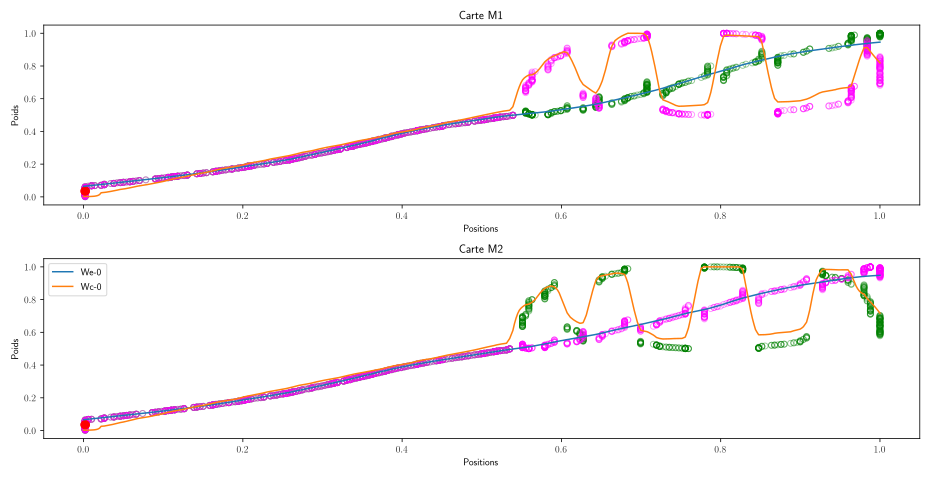
\includegraphics[width=\textwidth]{2som_mix_w.pdf}
	\caption{Représentation cartographique des poids et entrées pour la disposition mix}
	\end{minipage}
	\begin{minipage}{0.33\textwidth}
		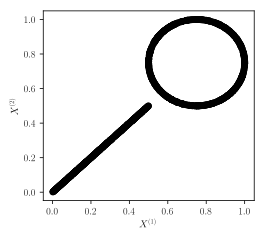
\includegraphics[width=\textwidth]{2som_mix_in.pdf}
	\end{minipage}
\end{figure}

\begin{figure}
	\begin{minipage}{0.66\textwidth}
		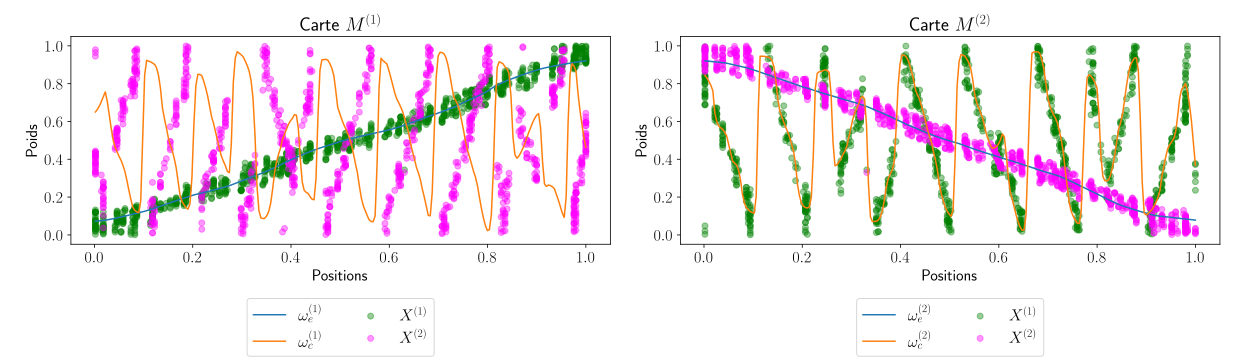
\includegraphics[width=\textwidth]{2som_square_w.pdf}
	\caption{Représentation cartographique des poids et entrées pour la disposition mix}
	\end{minipage}
	\begin{minipage}{0.33\textwidth}
		\includegraphics[width=\textwidth]{2som_square_in.pdf}
	\end{minipage}
\end{figure}


\begin{itemize}
	\item Organisation en zones dès que besoin de découpler deux valeurs de U
	\item Le comportement traduit l'existence de plusieurs valeurs de U pour une même entrée, sans forcément qu'une relation existe. Dans tous les cas, la carte effectue un découpage selon U.
	\item Lorsque relation il y a, ce découpage permet de faire de la prédiction.
\end{itemize}

\subsection{Conclusion}

Ces architectures de quelques cartes sont des architectures \emph{élémentaires}: toute architecture comportant plus de cartes pourra être construite à partir de petits modules. Nous considérerons les comportements observés dans ce chapitre comme des comportements élémentaires des architectures de cartes.


\section{Extension aux cartes en deux dimensions}

Nous avons étudié des comportements de base de cartes 1D sur des données en une dimension. Afin de généraliser le modèle à des données en dimension supérieures, nous avons cherché à observer ses propriétés d'auto-organisation, d'apprentissage et de prédiction sur des cartes en deux dimensions apprenant sur des données géométriques en 2D.
Les comportements d'une architecture de carte ont été mis en lumière sur des cartes 1D et des entrées 1D. Nous présentons dans cette section les comportements observés sur une architecture de deux cartes de type grille en deux dimensions. 

\subsection{Entrées}

Nous travaillons à présent sur des entrées en deux dimensions. Pour analyser un cas géométrique similaire au cas en une dimension, les entrées sont des points en 4 dimensions pour une structure de 2 cartes, 6 dimensions pour 3 cartes. Ces points sont situés sur une sphère 3D dont on a effectuée une rotation dans l'espace de plus haute dimension, de la même façon que les entrées en 3D se trouvaient sur un cercle 2D dont on a effectué une rotation dans l'espace, voir figure~\ref{fig:sphere_inputs}. La variable $U$ paramétrant cette surface est en deux dimensions.
Comme pour les entrées prises sur une courbe, nous normalisons les entrées entre 0 et 1 sur chaque dimension, entrainant une légère déformation de la courbe.
Nous prenons une architecture de deux cartes, prenant chacune une paire de dimensions du point en 4D (respectivement 6D).

\begin{figure}
	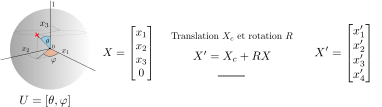
\includegraphics[width=\textwidth]{sphere_inputs.pdf}
	\caption{Transformation d'une surface d'un espace 3D en surface dans un espace 4D ou 6D. Les points restent positionnés sur une surface, mais sont plongés dans un espace de plus grande dimension. La rotation permet de répartir les coordonnées des points sur les dimensions. \label{fig:sphere_inputs}}
\end{figure}

\begin{figure}
	\begin{minipage}
		\centering\includegraphics[width=0.7\textwidth{2SOM_CUB_we_1999999.pdf}
	\end{minipage}
	\begin{minipage}
		\includegraphics[width=\textwidth{2SOM_CUB_wc_199999.pdf}
	\end{minipage}
	\caption{En haut: poids externes des cartes $M\m{1}$ et $M\m{2}$ représentés sous forme de distortion de la carte après 200000 itérations.
	En bas: poids contextuels des cartes pour la même itération, représentés sous forme de carte de couleur en deux dimensions. Un pixel situé à la position $p_i,p_j$ prend comme couleur correspondante la valeur 2D de son poids contextuel, associé à une couleur par la carte de coloration représentée à droite de la figure.
	On observe ici que les valeurs apprises  pour les poids contextuels restent autour de 0.5, et n'apprennent donc pas toutes les valeurs possibles des positions que prennent les BMU de sa carte voisine.}
	
	
\end{figure}


Ces cartes apprennent sur une sphere qui est "tournée" dans l'espace 4D, Ainsi, si on trace n'importe quel groupe de 3 coordonnées, ca fait un truc sphérique. Chaque carte prend deux coordonnées.
On a un U en 2 dimensions (coordonnées polaires d'une sphere)
Voici les vidéos des tracés des poids externes et contextuels (2D) de chaque carte.
Voici le tracé des erreurs de quantification dans chaque carte, ainsi que uv.
Il semble que bien qu'on retrouve le comportement en sous indices, on n'apprend pas spécialement de relations sur des cartes 2D. Selon moi, il faudrait d'explorer un grand nombre de paramètres pour éventuellement trouver un comportement émergeant. L'existence d'un tel comportement n'est pas exclu mais rien ne le garantit.

Remarques : dépliement des poids externes non assurés, et donc pb pour la relaxation

\section{Prédiction d'entrée}



\subsection{Entrées géométriques}


\subsection{Entrées réelles~: application sur un drône}


\section{Limites du modèle}


\ifSubfilesClassLoaded{
    \printbibliography
    %\externaldocument{../main.tex}   
}{}
\end{document}